\fancyhead{}
\fancyfoot{}
\cfoot{\thepage}

\lhead{Resultados}

\chapter{Resultados}

Este capítulo presenta el producto del análisis de los datos. Los resultados compendian el eventual tratamiento estadístico que se dio a los datos. Regularmente el orden es: a) análisis descriptivo de los datos, b) análisis inferenciales para responder a las preguntas de investigación y/o probar hipótesis. Según \cite{sampieri}, la American Psychological Association recomienda que primero se describa de manera breve la idea principal que resume los descubrimientos, y posteriormente se los reporten con detalle. Es importante destacar que en este capítulo no se incluyen conclusiones ni sugerencias, tampoco se deben explicar las implicaciones de la investigación. Esto se hace en el capítulo dedicado a la interpretaciones de los resultados, que en esta plantilla se denomina ``Discusión''.

Aquí el investigador se limita a describir sus hallazgos. Una manera útil de hacerlo es mediante elementos como tablas, gráficas, dibujos, diagramas, mapas y figuras generados por el análisis. Son elementos que sirven para organizar datos, de tal manera que el lector los pueda leer y entender las los vínculos entre las variables. Cada uno de dichos elementos debe ir enumerado. Una buena regla para elaborar una tabla es organizarla lógicamente y eliminar la información que pudiera confundir al lector.

Es conveniente brindar una sencilla explicación de las pruebas realizadas y presentar los resultados de la manera más comprensible posible. En este caso las tablas deben ser descritas. Los diagramas, figuras, mapas cognoscitivos, esquemas, matrices y otros elementos gráficos también deben ser numerados según una  lógica secuencial. Se debe observar el principio básico: una buena figura es sencilla, clara y no estorba la continuidad de la lectura. Las tablas, las figuras y los gráficos deben enriquecer el texto; en lugar de duplicarlos, deben comunicar los hechos esenciales, ser coherentes y fáciles de leer y comprender. 

\section{Ejemplos de elementos gráficos}

\textbf{Figuras y Tablas}

Las figuras y tablas deben insertarse en el punto apropiado dentro del texto.

Cada figura debe estar seguida de un epígrafe que la identifique, enumere y describa brevemente. Cada figura debe ser referenciada al menos una vez, a través de su número (Fig. \ref{fig:huella}).

\begin{figure}[H]
\begin{center}

\includegraphics[scale = .5]{./capitulo_04/huella}
\caption{Huella dactilar.}
\label{fig:huella}
\end{center}
\end{figure}

Es deseable que las figuras puedan ser interpretadas satisfactoriamente aún cuando sean impresas en blanco y negro. Esto se facilita mucho haciendo uso inteligente de la combinación de colores de forma que se consiga buen contraste entre los colores empleados, máxime si se trata de diagramas, en que a menudo es posible prescindir por completo de otros colores que el blanco y el negro, (como en la figura \ref{fig:termodin}).

\begin{figure}[H]
\begin{center}
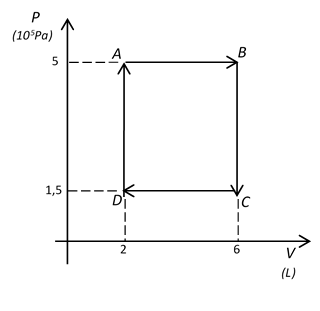
\includegraphics{./capitulo_04/termodin.png}
\caption{Ejemplificación de diagrama en blanco y negro.}
\label{fig:termodin}
\end{center}
\end{figure}

Las tablas deberían contener datos representativos que sinteticen información significativa del trabajo, evitando mostrar datos intermedios que pudieran dificultar la interpretación del mismo.

Cada tabla debe estar antecedida de un epígrafe que la identifique, enumere y describa brevemente.

Cada tabla debe ser referenciada al menos una vez, a través de su número, de preferencia antes de que aparezca en el documento, como en este caso (tabla \ref{tab:animales}).

\begin{table}[H]
\begin{center}
\caption{Inventario de animales.}
\label{tab:animales}
\begin{tabular}{||l|l|r||}
\hline
Especie&Sexo&Cantidad\\
\hline
\multirow{2}{*}{palomas}&jóvenes&20\\
&adultas&18\\
\hline
\multirow{2}{*}{conejos}&jóvenes&5\\
&adultos&5\\
\hline
\multirow{2}{*}{gallinas}&jóvenes&50\\
&adultas&50\\
\hline
\multicolumn{2}{||c|}{Total}&148\\
\hline
\end{tabular}
\end{center}
\end{table}

Otro ejemplo de tabla en el cual se observa el empleo de color, además de la combinación de columnas se observa en la tabla \ref{tab:color}

\begin{table}[H]
\begin{center}
\caption{Clasificación de la muestra, por edad.}
\label{tab:color}
\begin{tabular}{|c|cccc|}
\hline
\multirow{2}{*}{\cellcolor[rgb]{0.4,0.8,0.5}} &  \multicolumn{4}{>{\cellcolor[rgb]{0.4,0.8,0.9}}c|}{Tamaño de las muestras} \\ 
\cellcolor[rgb]{0.4,0.8,0.5}Edad&\cellcolor[rgb]{0.4,0.8,0.9} San Lorenzo &\cellcolor[rgb]{0.4,0.8,0.9} Asunción &\cellcolor[rgb]{0.4,0.8,0.9} Villarrica &\cellcolor[rgb]{0.4,0.8,0.9} Encarnación \\
\hline
e$<$20 &  93 &  74 &  68 & 87 \\
19$<$e$<$40 &  52 &  48 &  69 & 70 \\
39$<$e$<$60 &  47 &  85 &  81 & 64 \\
59$<$e$<$80 &  28 &  36 &  16 & 23 \\
79$<$e &  9 &  5 &  6 & 12 \\
\hline 
\end{tabular}
\end{center}
\end{table}

Aveces, como en el caso de la tabla \ref{tab:color}, el código se vuelve bastante complejo que resulta engorroso obtener en tiempo razonable la apariencia esperada de la tabla. En esos casos; es posible elaborar la tabla en entorno diferente a Latex; grabarla como imagen png, o jpg, o pdf; e insertarla enmascarada como tabla para ser contada como una de ellas por el contador de tablas: esto se logra con incluir la imagen dentro del entorno ``table'', como se ejemplifica con la tabla \ref{tab:tabla_word} que sigue.

\begin{table}[H]
	\begin{center}
		\caption{Imagen de tabla, en reemplazo de la tabla anterior.}
		\label{tab:tabla_word}
		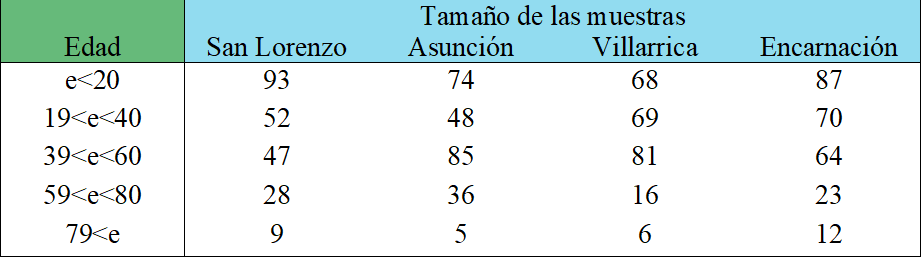
\includegraphics[scale=.65]{./capitulo_04/tabla_word.png}
	\end{center}
\end{table}

